
%(BEGIN_QUESTION)
% Copyright 2008, Tony R. Kuphaldt, released under the Creative Commons Attribution License (v 1.0)
% This means you may do almost anything with this work of mine, so long as you give me proper credit

The following table shows flow coefficients for three differently-characterized control valves as they are all stroked from 0\% (fully shut) to 100\% (fully open):

% No blank lines allowed between lines of an \halign structure!
% I use comments (%) instead, so that TeX doesn't choke.

$$\vbox{\offinterlineskip
\halign{\strut
\vrule \quad\hfil # \ \hfil & 
\vrule \quad\hfil # \ \hfil & 
\vrule \quad\hfil # \ \hfil & 
\vrule \quad\hfil # \ \hfil \vrule \cr
\noalign{\hrule}
%
% First row
Stem position & $C_v$ (Valve \#1) & $C_v$ (Valve \#2) & $C_v$ (Valve \#3) \cr
%
\noalign{\hrule}
%
% Another row
0 \% & 0.00 & 0.00 & 0.00 \cr
%
\noalign{\hrule}
%
% Another row
10 \% & 1.50 & 6.60 & 2.90 \cr
%
\noalign{\hrule}
%
% Another row
20 \% & 2.47 & 11.4 & 5.55 \cr
%
\noalign{\hrule}
%
% Another row
30 \% & 3.68 & 16.9 & 9.11 \cr
%
\noalign{\hrule}
%
% Another row
40 \% & 5.30 & 22.9 & 13.1 \cr
%
\noalign{\hrule}
%
% Another row
50 \% & 7.90 & 29.7 & 17.0 \cr
%
\noalign{\hrule}
%
% Another row
60 \% & 12.1 & 37.0 & 21.7 \cr
%
\noalign{\hrule}
%
% Another row
70 \% & 18.8 & 42.4 & 27.7 \cr
%
\noalign{\hrule}
%
% Another row
80 \% & 28.0 & 45.7 & 34.5 \cr
%
\noalign{\hrule}
%
% Another row
90 \% & 39.3 & 48.5 & 41.7 \cr
%
\noalign{\hrule}
%
% Another row
100 \% & 50.0 & 50.0 & 50.0 \cr
%
\noalign{\hrule}
} % End of \halign 
}$$ % End of \vbox

Plot all three valve characteristics on a graph and then identify which valve is quick-opening, which valve is linear, and which valve is equal-percentage.

\vfil 

\underbar{file i03214}
\eject
%(END_QUESTION)





%(BEGIN_ANSWER)

This is a graded question -- no answers or hints given!
 
%(END_ANSWER)





%(BEGIN_NOTES)

Valve \#1 is equal-percentage, valve \#2 is quick-opening, and valve \#3 is linear.

$$\includegraphics[width=15.5cm]{i03214x01.eps}$$

It is worthy to note here that the ``linear'' valve actually does {\it not} exhibit the straightest plot on this graph!  Only by comparing the three characteristic plots against each other may we tell for sure which one is linear (i.e. which one's plot lies between the two others).

\vskip 10pt

Data for the valve $C_v$ factors was derived from actual $C_v$ factors published in Fisher's ED, EAD, and EDR sliding-stem control valve product bulletin (51.1:ED).  I did not copy the exact data, however; I ``normalized'' the data so that all three valves would have the exact same full-open $C_v$ rating of 50.

%INDEX% Final Control Elements, valve: characterization

%(END_NOTES)


